\documentclass[xcolor=table]{beamer}       % flush equations
\usepackage[utf8]{inputenc}
\usepackage{mathtools}
\usepackage{amsmath}
\usepackage{ifthen}
\usepackage{array}
\usepackage{graphicx}               % picture support
\usepackage{multicol}
\usepackage{tikz}
\usetikzlibrary{positioning}
\usetikzlibrary{arrows}
\tikzstyle{arrow} = [thick,->,>=latex]
\newcommand*\circled[1]{\tikz[baseline=(char.base)]{
            \node[shape=circle,draw,inner sep=2pt] (char) {\tiny #1};}}

% BIB MANAGEMENT
\usepackage[
    style=authoryear-comp,
    maxbibnames=99,
    maxcitenames=2,
    uniquelist=false,
    giveninits,
    natbib
]{biblatex}
\addbibresource{../literature/bibliography.bib}
\newcommand{\poscite}[1]{\citeauthor{#1}'s (\citeyear{#1})}
% \hypersetup{
% colorlinks, %rather than outlining them in boxes
% linkcolor=blue, %override truly awful colour choices
% citecolor=blue, %(ditto)
% urlcolor=blue
% }

\newcommand*{\signed}[1]{%
  \unskip\hspace*{1em plus 1fill}%
  \nolinebreak[3]\hspace*{\fill}\mbox{#1}
}
\usepackage{csquotes}

\DeclareCiteCommand{\citeyear}
    {}
    {\bibhyperref{\printdate}}
    {\multicitedelim}
    {}

\usepackage{xcolor}
\definecolor{lightgray}{gray}{0.9}

\usepackage[T1]{fontenc}

% Fira Sans
\usepackage[sfdefault, scaled=.85, light]{FiraSans}
\usepackage{newtxsf}

% enable \pause in align environment
\makeatletter
\let\save@measuring@true\measuring@true
\def\measuring@true{%
  \save@measuring@true
  \def\beamer@sortzero##1{\beamer@ifnextcharospec{\beamer@sortzeroread{##1}}{}}%
  \def\beamer@sortzeroread##1<##2>{}%
  \def\beamer@finalnospec{}%
}
\makeatother

% use colors
\colorlet{fgblue}{blue!60!black}
\colorlet{bgred}{red!60!black}
\colorlet{fgred}{red!75!black}  % foreground must be brighter
\colorlet{mygrey}{black!10}  % foreground must be brighter
\newcommand{\red}[1]{\textcolor{fgred}{#1}}
\newcommand{\blue}[1]{\textcolor{fgblue}{#1}}

% use nice symbols
\usepackage{fontawesome5}

\mode<presentation>
{
    % general color theme:
    \usetheme{Madrid}
    \usecolortheme{beaver}
    % title page:
    \setbeamercolor   {title}     {bg=bgred, fg=white}
    \setbeamertemplate{title page}[default][rounded=true]
    % table of contents:
    \setbeamertemplate{section in toc}   [sections numbered]
    \setbeamertemplate{subsection in toc}[subsections numbered]
    % general style:
    \setbeamertemplate{navigation symbols}{} % no nav symbols
    \setbeamercolor{frametitle}         {bg=bgred, fg=white}
    \setbeamercolor{block title}        {bg=bgred, fg=white}
    \setbeamercolor{block title example}{bg=black!80, fg=fgred}
    \setbeamertemplate{blocks}[rounded] % blocks rounded, no shade
    % \setbeamercovered{transparent}: use within frame if wanted
    % lists:
        % enumerate
        \useinnertheme{rectangles}      % rectangular enumerate
        \setbeamercolor{item projected}   {bg=bgred}
        \setbeamercolor{enumerate item}   {bg=bgred, fg=white}
        \setbeamercolor{enumerate subitem}{bg=bgred, fg=white}
        % itemize
        \setbeamercolor{itemize item}   {fg=bgred}
        \setbeamercolor{itemize subitem}{fg=bgred}
        \setbeamertemplate{itemize item}   {$\blacktriangleright$}
        \setbeamertemplate{itemize subitem}{$\triangleright$}
        % description
        \setbeamercolor{description item}{fg=fgred}
}

% \AtBeginSection[]
% {
%     \begin{frame}
%     \frametitle{Outline}
%     \tableofcontents[hideothersubsections,currentsection]
%     \end{frame}
% }

% \AtBeginSubsection[]
% {
%     \begin{frame}
%     \frametitle{Outline}
%     \tableofcontents[hideothersubsections,currentsection,currentsubsection]
%     \end{frame}
% }

\usepackage{gb4e}

% title, author, day
\title[A Critical Analysis of the ATR]{A Critical Analysis of the Argumentative Theory of Reasoning:}
\subtitle{Caveats from the Evolution of Human Communication}
\author{Flip Lijnzaad}
\date{November 11, 2024}

\begin{document}

\maketitle

\begin{frame}{Introduction}
    \begin{itemize}
        \item Hugo Mercier and Dan Sperber
        \item Classically: function of reasoning is epistemic
        \item \alert{Argumentative} theory of reasoning:
            \\ the function of reasoning is to produce and evaluate arguments
    \begin{block}{\citet[p.~60]{MS11}}
        "Reasoning has evolved and persisted mainly because it makes human communication more effective and advantageous."
    \end{block}
    \end{itemize}
    \pause
    \begin{itemize}
        \item 'Function' in evolution
            \begin{itemize}
                \item Survival value
            \end{itemize}
    \end{itemize}
\end{frame}

\begin{frame}{Outline}
    \tableofcontents
\end{frame}

\section{The stability of communication}

\begin{frame}{The stability of communication}
    
\includegraphics[width=\textwidth]{img/stability-communication-1.png}
\end{frame}
\begin{frame}{The stability of communication}
    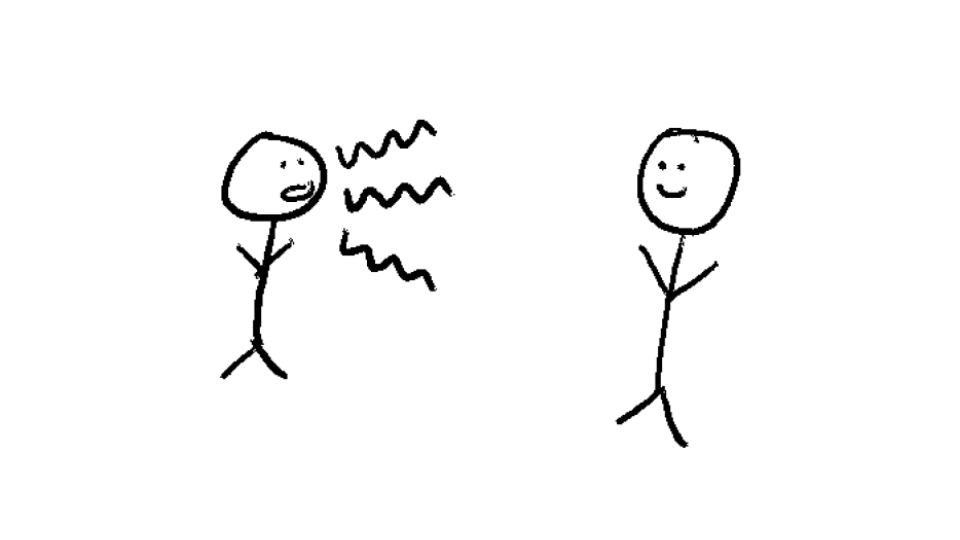
\includegraphics[width=\textwidth]{img/stability-communication-2.png}
\end{frame}
\begin{frame}{The stability of communication}
    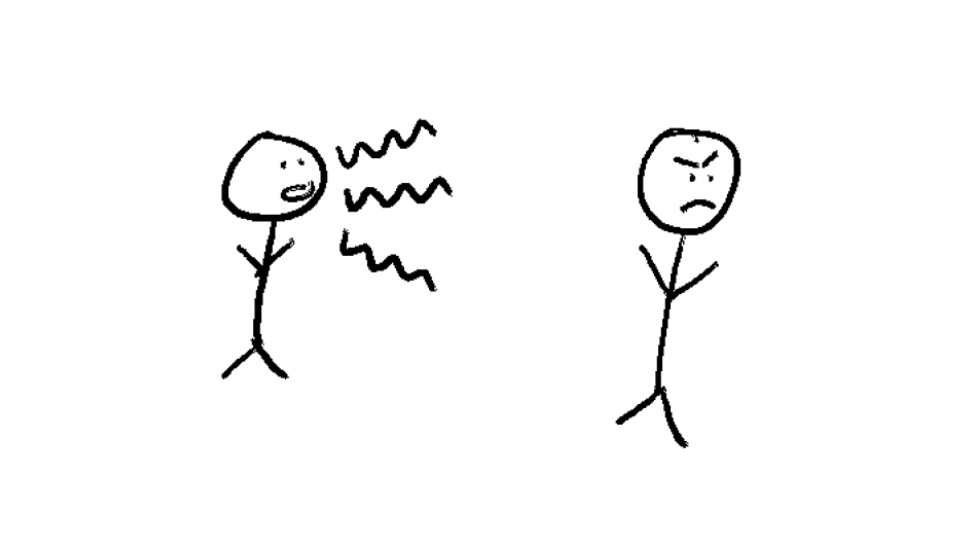
\includegraphics[width=\textwidth]{img/stability-communication-3.png}
\end{frame}
\begin{frame}{The stability of communication}
    
\includegraphics[width=\textwidth]{img/stability-communication-4.png}
\end{frame}

\begin{frame}{The evolutionary arms race}
    \centering
    \begin{tabular}{ccc}
        \textbf{sender} & & \textbf{receiver} \\ \\
        gain through deceiving \\
                        \pause & $\searrow$ & \\
                        & & coherence checking; \\ & & epistemic vigilance \\
                        \pause & $\swarrow$ \\
                        coherence display: \\ producing argument \\
                        \pause & $\searrow$ & \\
                        & & evaluating argument
    \end{tabular}
\end{frame}

\section{The argumentative theory of reasoning}

\begin{frame}{\insertsection}
    \begin{block}{\citet{MS11}}
    \begin{enumerate}
        \item Humans depend on cooperation; communication is crucial for this
        \item Communication must be advantageous for both senders and receivers
        \item It is advantageous to deceive, and disadvantageous to be deceived
    \end{enumerate}
    \pause
    \begin{itemize}
        \item Receivers exercise epistemic vigilance
        \item Senders produce arguments, evaluated by receivers
        \item Production and evaluation of arguments is facilitated by \alert{reasoning}
    \end{itemize}
    \end{block}
    \centering
    % \begin{tabular}{lll}
    %     \pause reasoning & facilitates & argumentation \\
    %     \pause argumentation & stabilizes & communication \\
    %     \pause communication & facilitates & cooperation \\
    %     \pause cooperation & contributes to & survival
    % \end{tabular}
    \pause reasoning
    \pause $\to$ argumentation
    \pause $\to$ communication
    \pause $\to$ cooperation
    \pause $\to$ survival
    \pause
    \medskip
    \begin{itemize}
        \item Empirical support
            \begin{itemize}
                \item Reasoning performance in argumentative settings
                \item Explanation of confirmation bias and motivated reasoning
            \end{itemize}
    \end{itemize}
\end{frame}

\section{Human communication and cooperation}

\begin{frame}{\insertsection}
    % emphasis:
    % * one bullet point about animals, one about children
    % * function of communication
    % * evolution of human cooperation
    % * some other minor takeaways in tomasello's work
    % * perhaps some ideas about lying
    \begin{itemize}
        \item Michael Tomasello
        \item Communication facilitates cooperation
        \item Function of cooperation
            \begin{itemize}
                \item Protection against predation
                \item Food sharing and shared labor in hunting and gathering
                \item Cooperative breeding
            \end{itemize}
        \item Evolution of human cooperation
            \begin{itemize}
                \item Obligate collaborators in gathering food
                \item Emergence of tolerance and trust
                \item Sophistication of collaborative skills $\to$ communication
                \item Mutual expectations become norms
                    % \begin{itemize}
                    %     \item Punishing norms violators
                    %     \item Social rationality: recognize dependence
                    % \end{itemize}
            \end{itemize}
    \end{itemize}
\end{frame}

\section{Criticizing the ATR}

\begin{frame}{\insertsection}
    % emphasis:
    % * function of communication
    % * trust or distrust as prior
    % * metatheoretical issues
    \begin{itemize}
        \item ATR is disconnected from broader context
        \item Cooperative function of communication
        \item Function of communication according to M\&S:
            \begin{itemize}
                \item For sender: causing 'desirable effects' $\to$ deception
                \item For receiver: gaining information
            \end{itemize}
        \item Underspecified from an evolutionary perspective
        \item Metatheoretical issues: vagueness in terminology and details
    \end{itemize}
\end{frame}

\begin{frame}{Selected bibliography}
    % \small
    \nocite{Scott-Phillips08, MS11, Tomasello09, Sperber01, Sperber10}
    % \nocite{Dor17}
    \printbibliography
\end{frame}

\end{document}
